% Generated by ic_study.analysis.v4_report_export from the v4 report with
% manifest SHA-256 6608b3960eb73011caca97870a4ffd3dbfbcd4c2df09bbbcb576c1c9452cf981.
% Edited during the journal revision (agent S, 2026-10-13): captions, headers and
% categorical cells in plain English; every number keeps its \resultnum binding.
\begin{table*}[tp]
\caption{Validation-gate outcomes from the sealed gate records: for each stage, tasks completed, task failures and criterion values against the prespecified criterion, with the stage verdict. Stages: zero-strength fitting check (G0), band calibration on synthetic scores (G1b), zero-strength band check (G1c), positive-strength dispersion check (G2) and nuisance-variance check (G2c); the identity unit tests (G1a) have no record in the gate (Section~\ref{sec:record-gate}). Each stage is read from its criteria line with the most completed tasks; every stage completed all its planned tasks. G2 cells carry the $(a,r)$ fixed by the second binding record; bracketed values are bootstrap intervals. The G1c summary, which the frozen runner could not write, is read from its successor record, computed by the frozen aggregating function. $V_{\mathrm{nuis}}/\mathrm{Var}_{\mathrm{refit}}$ (machine label Var\_D5/Var\_refit) is the locally propagated nuisance variance (decision item D5) divided by the variance of full refits. The covariance flag is a diagnostic added by revision v4.1 (item R3) and does not enter the criteria.}\label{tab:v4-T3}
\centering\scriptsize
\setlength{\tabcolsep}{2pt}
\begin{tabular}{p{2.2cm}p{4.0cm}p{2.9cm}p{3.0cm}}
\toprule
Stage & Item & Value & Criterion \\
\midrule
\raggedright Zero-strength fitting check (G0) & \raggedright tasks completed & \resultnum{v4.tab.T3.G0.tasks-completed.value.1}{81}/\resultnum{v4.tab.T3.G0.tasks-completed.value.2}{81} & all \\
\raggedright (passed) & \raggedright task failures & \resultnum{v4.tab.T3.G0.task-failures.value}{0} & = \resultnum{v4.tab.T3.G0.task-failures.criterion}{0} \\
 & \raggedright fits & \resultnum{v4.tab.T3.G0.fits.value}{648} &  \\
 & \raggedright a=\resultnum{v4.tab.T3.G0.a-0-identity-fits-not-anchor-exact.item}{0} fits of A, B, D, E and the B controls not anchor-exact & \resultnum{v4.tab.T3.G0.a-0-identity-fits-not-anchor-exact.value}{0} & = \resultnum{v4.tab.T3.G0.a-0-identity-fits-not-anchor-exact.criterion}{0} \\
 & \raggedright budget statuses & \resultnum{v4.tab.T3.G0.budget-statuses.value}{0} & = \resultnum{v4.tab.T3.G0.budget-statuses.criterion}{0} \\
 & \raggedright numerical-limit or ill-conditioned statuses / fits & \resultnum{v4.tab.T3.G0.implementation-statuses-fits.value.1}{2}/\resultnum{v4.tab.T3.G0.implementation-statuses-fits.value.2}{648} = \resultnum{v4.tab.T3.G0.implementation-statuses-fits.value.3}{0.0031} & $\leq$ \resultnum{v4.tab.T3.G0.implementation-statuses-fits.criterion}{0.01} \\
 & \raggedright status anchor-exact & \resultnum{v4.tab.T3.G0.status-anchor-exact.value}{63} & reported \\
 & \raggedright status family-limit-upper & \resultnum{v4.tab.T3.G0.status-family-limit-upper.value}{35} & reported \\
 & \raggedright status ill-conditioned & \resultnum{v4.tab.T3.G0.status-ill-conditioned.value}{2} & reported \\
 & \raggedright status interior & \resultnum{v4.tab.T3.G0.status-interior.value}{522} & reported \\
 & \raggedright status no-L1-root & \resultnum{v4.tab.T3.G0.status-no-L1-root.value}{22} & reported \\
 & \raggedright status non-monotone-profile & \resultnum{v4.tab.T3.G0.status-non-monotone-profile.value}{1} & reported \\
 & \raggedright status dependency gap & \resultnum{v4.tab.T3.G0.status-dependency-gap.value}{3} & reported \\
\raggedright Band calibration, synthetic scores (G1b) & \raggedright tasks completed & \resultnum{v4.tab.T3.G1b.tasks-completed.value.1}{5000}/\resultnum{v4.tab.T3.G1b.tasks-completed.value.2}{5000} & all \\
\raggedright (passed) & \raggedright task failures & \resultnum{v4.tab.T3.G1b.task-failures.value}{0} & = \resultnum{v4.tab.T3.G1b.task-failures.criterion}{0} \\
 & \raggedright joint coverage, Gaussian, ICC 0 & \resultnum{v4.tab.T3.G1b.joint-coverage-gaussian-icc0.value.1}{954}/\resultnum{v4.tab.T3.G1b.joint-coverage-gaussian-icc0.value.2}{1000} & $\geq$ \resultnum{v4.tab.T3.G1b.joint-coverage-gaussian-icc0.criterion.1}{935}/\resultnum{v4.tab.T3.G1b.joint-coverage-gaussian-icc0.criterion.2}{1000} \\
 & \raggedright joint coverage, Gaussian, ICC 0.5 & \resultnum{v4.tab.T3.G1b.joint-coverage-gaussian-icc05.value.1}{959}/\resultnum{v4.tab.T3.G1b.joint-coverage-gaussian-icc05.value.2}{1000} & $\geq$ \resultnum{v4.tab.T3.G1b.joint-coverage-gaussian-icc05.criterion.1}{935}/\resultnum{v4.tab.T3.G1b.joint-coverage-gaussian-icc05.criterion.2}{1000} \\
 & \raggedright joint coverage, $t_{5.2}$ clusters & \resultnum{v4.tab.T3.G1b.joint-coverage-non-gaussian.value.1}{954}/\resultnum{v4.tab.T3.G1b.joint-coverage-non-gaussian.value.2}{1000} & $\geq$ \resultnum{v4.tab.T3.G1b.joint-coverage-non-gaussian.criterion.1}{935}/\resultnum{v4.tab.T3.G1b.joint-coverage-non-gaussian.criterion.2}{1000} \\
 & \raggedright joint coverage, rounded ties & \resultnum{v4.tab.T3.G1b.joint-coverage-ties.value.1}{952}/\resultnum{v4.tab.T3.G1b.joint-coverage-ties.value.2}{1000} & $\geq$ \resultnum{v4.tab.T3.G1b.joint-coverage-ties.criterion.1}{935}/\resultnum{v4.tab.T3.G1b.joint-coverage-ties.criterion.2}{1000} \\
 & \raggedright joint coverage, cross-slot dependence & \resultnum{v4.tab.T3.G1b.joint-coverage-dependent-slots.value.1}{974}/\resultnum{v4.tab.T3.G1b.joint-coverage-dependent-slots.value.2}{1000} & $\geq$ \resultnum{v4.tab.T3.G1b.joint-coverage-dependent-slots.criterion.1}{935}/\resultnum{v4.tab.T3.G1b.joint-coverage-dependent-slots.criterion.2}{1000} \\
 & \raggedright empirical max-t above \resultnum{v4.tab.T3.G1b.empirical-max-t-above-2-7729.item}{2.7729} & \resultnum{v4.tab.T3.G1b.empirical-max-t-above-2-7729.value.1}{1363}/\resultnum{v4.tab.T3.G1b.empirical-max-t-above-2-7729.value.2}{5000} & reported \\
\raggedright Zero-strength band check (G1c) & \raggedright tasks completed & \resultnum{v4.tab.T3.G1c.tasks-completed.value.1}{150}/\resultnum{v4.tab.T3.G1c.tasks-completed.value.2}{150} & all \\
\raggedright (passed) & \raggedright task failures & \resultnum{v4.tab.T3.G1c.task-failures.value}{0} & = \resultnum{v4.tab.T3.G1c.task-failures.criterion}{0} \\
 & \raggedright summary source & successor record (frozen aggregate) &  \\
 & \raggedright anchor-exact fits & \resultnum{v4.tab.T3.G1c.anchor-exact-fits.value.1}{150}/\resultnum{v4.tab.T3.G1c.anchor-exact-fits.value.2}{150} & = \resultnum{v4.tab.T3.G1c.anchor-exact-fits.criterion.1}{150}/\resultnum{v4.tab.T3.G1c.anchor-exact-fits.criterion.2}{150} \\
 & \raggedright pointwise failures at \resultnum{v4.tab.T3.G1c.pointwise-failures-at-2-7729.item}{2.7729} & \resultnum{v4.tab.T3.G1c.pointwise-failures-at-2-7729.value.1}{1}/\resultnum{v4.tab.T3.G1c.pointwise-failures-at-2-7729.value.2}{150} & $\leq$ \resultnum{v4.tab.T3.G1c.pointwise-failures-at-2-7729.criterion}{3} \\
 & \raggedright $|$mean AUC - \resultnum{v4.tab.T3.G1c.mean-AUC-0-5-SE.item}{0.5}$|$ / SE & \resultnum{v4.tab.T3.G1c.mean-AUC-0-5-SE.value}{0.376} & $\leq$ \resultnum{v4.tab.T3.G1c.mean-AUC-0-5-SE.criterion}{3} \\
 & \raggedright tie rate & \resultnum{v4.tab.T3.G1c.tie-rate.value}{0.0000} & reported \\
\botrule
\end{tabular}
\end{table*}
\begin{table*}[tp]
\addtocounter{table}{-\csname @ne\endcsname}
\providecommand{\theHtable}{\thetable}
\renewcommand{\theHtable}{v4-T3-part1}
\caption{Validation-gate outcomes (continued)}\label{tab:v4-T3-part1}
\centering\scriptsize
\setlength{\tabcolsep}{2pt}
\begin{tabular}{p{2.2cm}p{4.0cm}p{2.9cm}p{3.0cm}}
\toprule
Stage & Item & Value & Criterion \\
\midrule
\raggedright Positive-strength dispersion check (G2) & \raggedright tasks completed & \resultnum{v4.tab.T3.G2.tasks-completed.value.1}{700}/\resultnum{v4.tab.T3.G2.tasks-completed.value.2}{700} & all \\
\raggedright (passed) & \raggedright task failures & \resultnum{v4.tab.T3.G2.task-failures.value}{0} & $\leq$ \resultnum{v4.tab.T3.G2.task-failures.criterion}{2}\% pooled \\
 & \raggedright dispersion ratio, cell \resultnum{v4.tab.T3.G2.dispersion-ratio-cell-1-a-0-003-r-0-70.item.1}{1} (a=\resultnum{v4.tab.T3.G2.dispersion-ratio-cell-1-a-0-003-r-0-70.item.2}{0.003}, r=\resultnum{v4.tab.T3.G2.dispersion-ratio-cell-1-a-0-003-r-0-70.item.3}{0.70}) & \resultnum{v4.tab.T3.G2.dispersion-ratio-cell-1-a-0-003-r-0-70.value.1}{0.658} [\resultnum{v4.tab.T3.G2.dispersion-ratio-cell-1-a-0-003-r-0-70.value.2}{0.462}, \resultnum{v4.tab.T3.G2.dispersion-ratio-cell-1-a-0-003-r-0-70.value.3}{0.841}] & upper $\geq$ \resultnum{v4.tab.T3.G2.dispersion-ratio-cell-1-a-0-003-r-0-70.criterion.1}{0.498}, lower $\leq$ \resultnum{v4.tab.T3.G2.dispersion-ratio-cell-1-a-0-003-r-0-70.criterion.2}{1.288} \\
 & \raggedright dispersion ratio, cell \resultnum{v4.tab.T3.G2.dispersion-ratio-cell-2-a-0-01-r-0-70.item.1}{2} (a=\resultnum{v4.tab.T3.G2.dispersion-ratio-cell-2-a-0-01-r-0-70.item.2}{0.01}, r=\resultnum{v4.tab.T3.G2.dispersion-ratio-cell-2-a-0-01-r-0-70.item.3}{0.70}) & \resultnum{v4.tab.T3.G2.dispersion-ratio-cell-2-a-0-01-r-0-70.value.1}{0.837} [\resultnum{v4.tab.T3.G2.dispersion-ratio-cell-2-a-0-01-r-0-70.value.2}{0.545}, \resultnum{v4.tab.T3.G2.dispersion-ratio-cell-2-a-0-01-r-0-70.value.3}{1.131}] & upper $\geq$ \resultnum{v4.tab.T3.G2.dispersion-ratio-cell-2-a-0-01-r-0-70.criterion.1}{0.498}, lower $\leq$ \resultnum{v4.tab.T3.G2.dispersion-ratio-cell-2-a-0-01-r-0-70.criterion.2}{1.288} \\
 & \raggedright dispersion ratio, cell \resultnum{v4.tab.T3.G2.dispersion-ratio-cell-3-a-0-03-r-0-70.item.1}{3} (a=\resultnum{v4.tab.T3.G2.dispersion-ratio-cell-3-a-0-03-r-0-70.item.2}{0.03}, r=\resultnum{v4.tab.T3.G2.dispersion-ratio-cell-3-a-0-03-r-0-70.item.3}{0.70}) & \resultnum{v4.tab.T3.G2.dispersion-ratio-cell-3-a-0-03-r-0-70.value.1}{0.640} [\resultnum{v4.tab.T3.G2.dispersion-ratio-cell-3-a-0-03-r-0-70.value.2}{0.389}, \resultnum{v4.tab.T3.G2.dispersion-ratio-cell-3-a-0-03-r-0-70.value.3}{0.910}] & upper $\geq$ \resultnum{v4.tab.T3.G2.dispersion-ratio-cell-3-a-0-03-r-0-70.criterion.1}{0.498}, lower $\leq$ \resultnum{v4.tab.T3.G2.dispersion-ratio-cell-3-a-0-03-r-0-70.criterion.2}{1.288} \\
 & \raggedright dispersion ratio, cell \resultnum{v4.tab.T3.G2.dispersion-ratio-cell-4-a-0-1-r-0-70.item.1}{4} (a=\resultnum{v4.tab.T3.G2.dispersion-ratio-cell-4-a-0-1-r-0-70.item.2}{0.1}, r=\resultnum{v4.tab.T3.G2.dispersion-ratio-cell-4-a-0-1-r-0-70.item.3}{0.70}) & \resultnum{v4.tab.T3.G2.dispersion-ratio-cell-4-a-0-1-r-0-70.value.1}{1.346} [\resultnum{v4.tab.T3.G2.dispersion-ratio-cell-4-a-0-1-r-0-70.value.2}{0.870}, \resultnum{v4.tab.T3.G2.dispersion-ratio-cell-4-a-0-1-r-0-70.value.3}{1.821}] & upper $\geq$ \resultnum{v4.tab.T3.G2.dispersion-ratio-cell-4-a-0-1-r-0-70.criterion.1}{0.498}, lower $\leq$ \resultnum{v4.tab.T3.G2.dispersion-ratio-cell-4-a-0-1-r-0-70.criterion.2}{1.288} \\
 & \raggedright dispersion ratio, cell \resultnum{v4.tab.T3.G2.dispersion-ratio-cell-5-a-0-3-r-0-70.item.1}{5} (a=\resultnum{v4.tab.T3.G2.dispersion-ratio-cell-5-a-0-3-r-0-70.item.2}{0.3}, r=\resultnum{v4.tab.T3.G2.dispersion-ratio-cell-5-a-0-3-r-0-70.item.3}{0.70}) & \resultnum{v4.tab.T3.G2.dispersion-ratio-cell-5-a-0-3-r-0-70.value.1}{0.934} [\resultnum{v4.tab.T3.G2.dispersion-ratio-cell-5-a-0-3-r-0-70.value.2}{0.557}, \resultnum{v4.tab.T3.G2.dispersion-ratio-cell-5-a-0-3-r-0-70.value.3}{1.315}] & upper $\geq$ \resultnum{v4.tab.T3.G2.dispersion-ratio-cell-5-a-0-3-r-0-70.criterion.1}{0.498}, lower $\leq$ \resultnum{v4.tab.T3.G2.dispersion-ratio-cell-5-a-0-3-r-0-70.criterion.2}{1.288} \\
 & \raggedright dispersion ratio, cell \resultnum{v4.tab.T3.G2.dispersion-ratio-cell-6-a-0-03-r-0-50.item.1}{6} (a=\resultnum{v4.tab.T3.G2.dispersion-ratio-cell-6-a-0-03-r-0-50.item.2}{0.03}, r=\resultnum{v4.tab.T3.G2.dispersion-ratio-cell-6-a-0-03-r-0-50.item.3}{0.50}) & \resultnum{v4.tab.T3.G2.dispersion-ratio-cell-6-a-0-03-r-0-50.value.1}{1.040} [\resultnum{v4.tab.T3.G2.dispersion-ratio-cell-6-a-0-03-r-0-50.value.2}{0.773}, \resultnum{v4.tab.T3.G2.dispersion-ratio-cell-6-a-0-03-r-0-50.value.3}{1.303}] & upper $\geq$ \resultnum{v4.tab.T3.G2.dispersion-ratio-cell-6-a-0-03-r-0-50.criterion.1}{0.498}, lower $\leq$ \resultnum{v4.tab.T3.G2.dispersion-ratio-cell-6-a-0-03-r-0-50.criterion.2}{1.288} \\
 & \raggedright dispersion ratio, cell \resultnum{v4.tab.T3.G2.dispersion-ratio-cell-7-a-0-03-r-0-90.item.1}{7} (a=\resultnum{v4.tab.T3.G2.dispersion-ratio-cell-7-a-0-03-r-0-90.item.2}{0.03}, r=\resultnum{v4.tab.T3.G2.dispersion-ratio-cell-7-a-0-03-r-0-90.item.3}{0.90}) & \resultnum{v4.tab.T3.G2.dispersion-ratio-cell-7-a-0-03-r-0-90.value.1}{1.303} [\resultnum{v4.tab.T3.G2.dispersion-ratio-cell-7-a-0-03-r-0-90.value.2}{0.840}, \resultnum{v4.tab.T3.G2.dispersion-ratio-cell-7-a-0-03-r-0-90.value.3}{1.786}] & upper $\geq$ \resultnum{v4.tab.T3.G2.dispersion-ratio-cell-7-a-0-03-r-0-90.criterion.1}{0.498}, lower $\leq$ \resultnum{v4.tab.T3.G2.dispersion-ratio-cell-7-a-0-03-r-0-90.criterion.2}{1.288} \\
 & \raggedright dispersion ratio, pooled & \resultnum{v4.tab.T3.G2.dispersion-ratio-pooled.value.1}{0.971} [\resultnum{v4.tab.T3.G2.dispersion-ratio-pooled.value.2}{0.760}, \resultnum{v4.tab.T3.G2.dispersion-ratio-pooled.value.3}{1.125}] & upper $\geq$ \resultnum{v4.tab.T3.G2.dispersion-ratio-pooled.criterion.1}{0.818}, lower $\leq$ \resultnum{v4.tab.T3.G2.dispersion-ratio-pooled.criterion.2}{1.055} \\
 & \raggedright failures by cell & \resultnum{v4.tab.T3.G2.failures-by-cell.value.1}{0} \resultnum{v4.tab.T3.G2.failures-by-cell.value.2}{0} \resultnum{v4.tab.T3.G2.failures-by-cell.value.3}{0} \resultnum{v4.tab.T3.G2.failures-by-cell.value.4}{0} \resultnum{v4.tab.T3.G2.failures-by-cell.value.5}{0} \resultnum{v4.tab.T3.G2.failures-by-cell.value.6}{0} \resultnum{v4.tab.T3.G2.failures-by-cell.value.7}{0} & $\leq$ \resultnum{v4.tab.T3.G2.failures-by-cell.criterion.1}{5} per cell; $\leq$ \resultnum{v4.tab.T3.G2.failures-by-cell.criterion.2}{2}\% pooled \\
 & \raggedright median finite-difference variance ratio by cell & \resultnum{v4.tab.T3.G2.FD-variance-ratio-median-by-cell.value.1}{0.972} \resultnum{v4.tab.T3.G2.FD-variance-ratio-median-by-cell.value.2}{0.951} \resultnum{v4.tab.T3.G2.FD-variance-ratio-median-by-cell.value.3}{0.993} \resultnum{v4.tab.T3.G2.FD-variance-ratio-median-by-cell.value.4}{1.000} \resultnum{v4.tab.T3.G2.FD-variance-ratio-median-by-cell.value.5}{0.983} \resultnum{v4.tab.T3.G2.FD-variance-ratio-median-by-cell.value.6}{0.976} \resultnum{v4.tab.T3.G2.FD-variance-ratio-median-by-cell.value.7}{0.986} & each in [\resultnum{v4.tab.T3.G2.FD-variance-ratio-median-by-cell.criterion.1}{0.8}, \resultnum{v4.tab.T3.G2.FD-variance-ratio-median-by-cell.criterion.2}{1.25}] \\
 & \raggedright leave-one-out tail counts by cell & \resultnum{v4.tab.T3.G2.LOO-tail-counts-by-cell.value.1}{0} \resultnum{v4.tab.T3.G2.LOO-tail-counts-by-cell.value.2}{0} \resultnum{v4.tab.T3.G2.LOO-tail-counts-by-cell.value.3}{0} \resultnum{v4.tab.T3.G2.LOO-tail-counts-by-cell.value.4}{0} \resultnum{v4.tab.T3.G2.LOO-tail-counts-by-cell.value.5}{0} \resultnum{v4.tab.T3.G2.LOO-tail-counts-by-cell.value.6}{0} \resultnum{v4.tab.T3.G2.LOO-tail-counts-by-cell.value.7}{0} & reported \\
 & \raggedright covariance flags by cell & \resultnum{v4.tab.T3.G2.covariance-flags-by-cell.value.1}{0} \resultnum{v4.tab.T3.G2.covariance-flags-by-cell.value.2}{0} \resultnum{v4.tab.T3.G2.covariance-flags-by-cell.value.3}{0} \resultnum{v4.tab.T3.G2.covariance-flags-by-cell.value.4}{0} \resultnum{v4.tab.T3.G2.covariance-flags-by-cell.value.5}{17} \resultnum{v4.tab.T3.G2.covariance-flags-by-cell.value.6}{0} \resultnum{v4.tab.T3.G2.covariance-flags-by-cell.value.7}{0} & reported (diagnostic) \\
\raggedright Nuisance-variance check (G2c) & \raggedright tasks completed & \resultnum{v4.tab.T3.G2c.tasks-completed.value.1}{142}/\resultnum{v4.tab.T3.G2c.tasks-completed.value.2}{142} & all \\
\raggedright (passed) & \raggedright task failures & \resultnum{v4.tab.T3.G2c.task-failures.value}{0} & per comparison \\
 & \raggedright $V_{\mathrm{nuis}}/\mathrm{Var}_{\mathrm{refit}}$, a=\resultnum{v4.tab.T3.G2c.Var-D5-Var-refit-a-0-10-100-refits.item.1}{0.10}, \resultnum{v4.tab.T3.G2c.Var-D5-Var-refit-a-0-10-100-refits.item.2}{100} refits & \resultnum{v4.tab.T3.G2c.Var-D5-Var-refit-a-0-10-100-refits.value.1}{1.117} [\resultnum{v4.tab.T3.G2c.Var-D5-Var-refit-a-0-10-100-refits.value.2}{0.912}, \resultnum{v4.tab.T3.G2c.Var-D5-Var-refit-a-0-10-100-refits.value.3}{1.493}] & upper $\geq$ \resultnum{v4.tab.T3.G2c.Var-D5-Var-refit-a-0-10-100-refits.criterion.1}{0.8}, lower $\leq$ \resultnum{v4.tab.T3.G2c.Var-D5-Var-refit-a-0-10-100-refits.criterion.2}{2.0} \\
 & \raggedright refit failures, a=\resultnum{v4.tab.T3.G2c.refit-failures-a-0-10-100-refits.item.1}{0.10}, \resultnum{v4.tab.T3.G2c.refit-failures-a-0-10-100-refits.item.2}{100} refits & \resultnum{v4.tab.T3.G2c.refit-failures-a-0-10-100-refits.value.1}{0}/\resultnum{v4.tab.T3.G2c.refit-failures-a-0-10-100-refits.value.2}{100} & $\leq$ \resultnum{v4.tab.T3.G2c.refit-failures-a-0-10-100-refits.criterion.1}{3}/\resultnum{v4.tab.T3.G2c.refit-failures-a-0-10-100-refits.criterion.2}{100} \\
 & \raggedright refit tail counts, a=\resultnum{v4.tab.T3.G2c.refit-tails-a-0-10-100-refits.item.1}{0.10}, \resultnum{v4.tab.T3.G2c.refit-tails-a-0-10-100-refits.item.2}{100} refits & \resultnum{v4.tab.T3.G2c.refit-tails-a-0-10-100-refits.value}{0} & reported \\
 & \raggedright $V_{\mathrm{nuis}}/\mathrm{Var}_{\mathrm{refit}}$, a=\resultnum{v4.tab.T3.G2c.Var-D5-Var-refit-a-0-03-40-refits.item.1}{0.03}, \resultnum{v4.tab.T3.G2c.Var-D5-Var-refit-a-0-03-40-refits.item.2}{40} refits & \resultnum{v4.tab.T3.G2c.Var-D5-Var-refit-a-0-03-40-refits.value.1}{0.629} [\resultnum{v4.tab.T3.G2c.Var-D5-Var-refit-a-0-03-40-refits.value.2}{0.470}, \resultnum{v4.tab.T3.G2c.Var-D5-Var-refit-a-0-03-40-refits.value.3}{0.931}] & upper $\geq$ \resultnum{v4.tab.T3.G2c.Var-D5-Var-refit-a-0-03-40-refits.criterion.1}{0.8}, lower $\leq$ \resultnum{v4.tab.T3.G2c.Var-D5-Var-refit-a-0-03-40-refits.criterion.2}{2.0} \\
 & \raggedright refit failures, a=\resultnum{v4.tab.T3.G2c.refit-failures-a-0-03-40-refits.item.1}{0.03}, \resultnum{v4.tab.T3.G2c.refit-failures-a-0-03-40-refits.item.2}{40} refits & \resultnum{v4.tab.T3.G2c.refit-failures-a-0-03-40-refits.value.1}{0}/\resultnum{v4.tab.T3.G2c.refit-failures-a-0-03-40-refits.value.2}{40} & $\leq$ \resultnum{v4.tab.T3.G2c.refit-failures-a-0-03-40-refits.criterion.1}{2}/\resultnum{v4.tab.T3.G2c.refit-failures-a-0-03-40-refits.criterion.2}{40} \\
 & \raggedright refit tail counts, a=\resultnum{v4.tab.T3.G2c.refit-tails-a-0-03-40-refits.item.1}{0.03}, \resultnum{v4.tab.T3.G2c.refit-tails-a-0-03-40-refits.item.2}{40} refits & \resultnum{v4.tab.T3.G2c.refit-tails-a-0-03-40-refits.value}{0} & reported \\
\botrule
\end{tabular}
\end{table*}
\begin{figure}[tp]
\centering
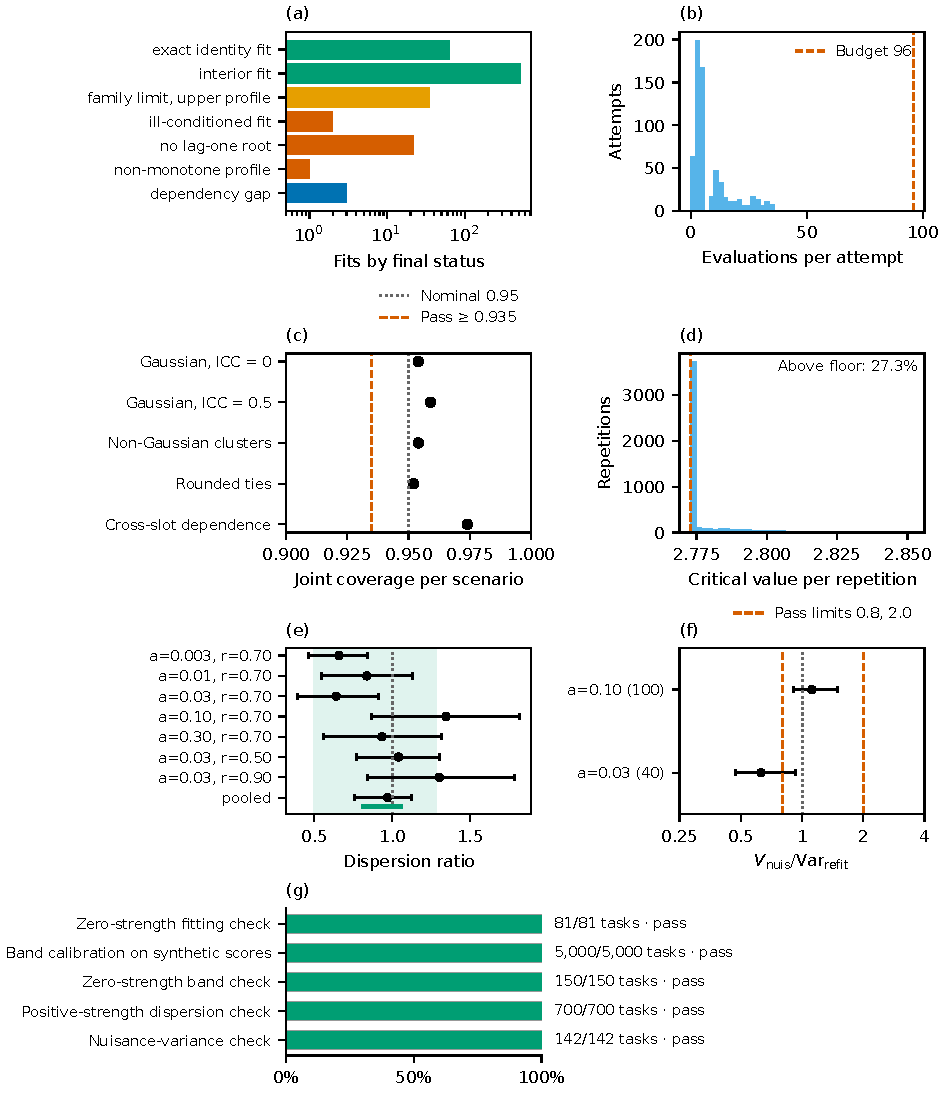
\includegraphics[width=\textwidth,height=150mm,keepaspectratio]{generated/J4_gate_diagnostics.pdf}
\caption{Validation-gate diagnostics from the public aggregates: (a) final fit statuses and (b) solver evaluations per attempt in the zero-strength fitting check (budget \resultnum{j.gate.solver_budget}{96}); (c) joint coverage per scenario and (d) critical values in the band calibration on synthetic scores, with the pass mark, nominal level and critical-value floor \resultnum{j.gate.critical_floor}{2.7729}; (e) dispersion ratios in the positive-strength dispersion check with bootstrap intervals and calibrated cell (shading) and pooled (green segment) thresholds; (f) local nuisance-variance estimates relative to full refits in the nuisance-variance check, with one-sided bounds; (g) completed tasks and verdict by stage. Family limits are gaps. The zero-strength band check uses its corrected aggregate record.}\label{fig:gate-diagnostics}
\end{figure}

